%% LaTeX2e class for student theses
%% thesis.tex
%%
%% Karlsruhe University of Applied Sciences
%% Faculty of  Computer Science and Business Information Systems
%%
%%
%% Version 0.2, 2017-11-15
%%
%% --------------------------------------------------------
%% | Derived from sdqthesis by Erik Burger burger@kit.edu |
%% --------------------------------------------------------

%% Available languages: english,ngerman
%% Available modes: draft,final (see README)
\documentclass[english,final]{thesis}

% Use space between paragraphs
%\KOMAoption{parskip}{half+}

%% ---------------------------------
%% | Information about the thesis  |
%% ---------------------------------

%% Name of the author
\author{Julian Bücher}

%% Title (and possibly subtitle) of the thesis
\title{Reservation process for charging infrastructure management in the context of e-mobility}

%% Type of the thesis
\thesistype{Master Thesis}

%% Change the institute or subject area here, ``VSYS'' is default
% \myinstitute{Institute for \dots}

%% You can put a logo in the ``logos'' directory and include it here
% \grouplogo{myfile}

%% The reviewers are the professors that grade your thesis , ``Zirpins'' is default
\reviewerone{Prof. Dr.-Ing. Zoltán Nochta}
%% reviewer two (can be omitted)
\reviewertwo{Prof. Dr. rer. nat. Heiko Körner}

%% The advisor is usually extern (can be omitted)
% \advisorone{Dipl.-Inform. C}
% The second advisor (can be omitted)
% \advisortwo{Dipl.-Inform. D}


%% Please enter the start end end time of your thesis
\editingtime{17. March 2023}{16. September 2023}

\settitle

%% --------------------------------
%% | Settings for word separation |
%% --------------------------------

%% Describe separation hints here.
%% For more details, see
%% http://en.wikibooks.org/wiki/LaTeX/Text_Formatting#Hyphenation
\hyphenation{
% me-ta-mo-del
}

%% --------------------------------
%% | Bibliography                 |
%% --------------------------------

%% Use biber instead of BibTeX, see README
\usepackage[citestyle=numeric,style=numeric,backend=biber]{biblatex}
\addbibresource{thesis.bib}

%% --------------------------------
%% | Listings                     |
%% --------------------------------

%% Basic config
\lstset{
  frame=tb,
  aboveskip=3mm,
  belowskip=3mm,
  showstringspaces=false,
  columns=flexible,
  basicstyle={\footnotesize\ttfamily},
  numbers=left,
  numberstyle=\tiny\color{gray},
  keywordstyle=\color{blue},
  commentstyle=\color{dkgreen},
  stringstyle=\color{mauve},
  breaklines=true,
  breakatwhitespace=true,
  tabsize=3,
  showlines=true
}

%% Add your non-supported language here
\lstdefinelanguage{JavaScript}{
  keywords={typeof, new, true, false, catch, function, return, null, catch, switch, var, if, in, while, do, else, case, break},
  keywordstyle=\color{blue}\bfseries,
  ndkeywords={class, export, boolean, throw, implements, import, this},
  ndkeywordstyle=\color{darkgray}\bfseries,
  identifierstyle=\color{black},
  sensitive=false,
  comment=[l]{//},
  morecomment=[s]{/*}{*/},
  commentstyle=\color{purple}\ttfamily,
  stringstyle=\color{red}\ttfamily,
  morestring=[b]',
  morestring=[b]"
}

%% --------------------------------
%% | Glossaries                   |
%% --------------------------------

%% Use glossaries (optional)
\makeglossaries
%% Load glossary definitions from file
\loadglsentries{glossentries.tex}

%% ====================================
%% ====================================
%% ||                                ||
%% || Beginning of the main document ||
%% ||                                ||
%% ====================================
%% ====================================
\begin{document}

%% Set PDF metadata
\setpdf

%% Set the title
\maketitle

%% The Preamble begins here
\frontmatter

%% LaTeX2e class for student theses: Declaration of independent work
%% sections/declaration.tex
%%
%% Karlsruhe University of Applied Sciences
%% Faculty of  Computer Science and Business Information Systems
%%
%% --------------------------------------------------------
%% | Derived from sdqthesis by Erik Burger burger@kit.edu |
%% --------------------------------------------------------


\thispagestyle{empty}
\null\vfill
\noindent\hbox to \textwidth{\hrulefill}
\iflanguage{english}{I declare that I have developed and written the enclosed
thesis completely by myself, and have not used sources or means without
declaration in the text.}%
{Ich versichere wahrheitsgemäß, die Arbeit
selbstständig angefertigt, alle benutzten Hilfsmittel vollständig und genau
angegeben und alles kenntlich gemacht zu haben, was aus Arbeiten anderer
unverändert oder mit Änderungen entnommen wurde.}


%% ---------------------------------------------
%% | Replace PLACE and DATE with actual values |
%% ---------------------------------------------
\textbf{Karlsruhe, 16.09.2023}
\vspace{1.5cm}

\dotfill\hspace*{8.0cm}\\
\hspace*{2cm}(\theauthor)
\cleardoublepage


\setcounter{page}{1}
\pagenumbering{roman}

%% ----------------
%% |   Abstract   |
%% ----------------

%% For theses written in English, an abstract both in English
%% and German is mandatory.
%%
%% For theses written in German, a German abstract is sufficient.
%%
%% The text is included from the following files:
%% - sections/abstract

\includeabstract

%% ------------------------
%% |   Table of Contents  |
%% ------------------------
\tableofcontents

\listoffigures
\listoftables

%% ------------------------
%% | Glossary/Acronyms    |
%% ------------------------

% print glossary (optional)
\printglossary[title=Glossar]

% print acronyms (optional)
\printglossary[type=\acronymtype]

%% -----------------
%% |   Main part   |
%% -----------------

\mainmatter
% Introduction
%% LaTeX2e class for student theses
%% sections/introduction/content.tex
%%
%% Karlsruhe University of Applied Sciences
%% Faculty of  Computer Science and Business Information Systems
%%
%% --------------------------------------------------------
%% | Derived from sdqthesis by Erik Burger burger@kit.edu |
%% --------------------------------------------------------

\chapter{Introduction}
\label{ch:Introduction}

% E-Mobility and Reservations...

\section{Target}
\label{ch:Introduction:sec:Target}

The fact that subsidies and other inducements provided by the manufacturers and the state itself lead to an further increasing amount of electric vehicles \cite{afshar_literature_2020} on the streets, the extension and management of the existing charging infrastructure will become an essential part of the overall satisfaction of the \acrfull{evu} community.
Especially management or administration processes ensuring a fair and well-regulated use of the single charging possibilities is a necessary feature most implementations are missing nowadays. 
The prime example addressing this problem, is the feature gap describing a reservation of a charging point in a specified time in the future. 

Therefore reservation process for electric vehicle management inside a reduced scenario, like a company car fleet, will be used as proof of concept to demonstrate the advantages in comparison to the first-come-first-serve principle. The following sections will describe the context of the required system with their given requirements and restrictions for the tasks. First of all, a definition for electric mobility will be given, which declares the given context and its parts.

\section{SAP SE}
\label{ch:Introduction:sec:SAP SE}
SAP SE, commonly referred to as SAP, is a multinational software corporation based in Walldorf, Germany. It is one of the world's leading enterprise software companies and is renowned for its innovative solutions that help businesses manage their operations effectively. It was founded in 1972 by Dietmar Hopp, Hasso Plattner, Claus Wellenreuther, Hans-Werner Hector, and Klaus Tschira. The company's primary goal was to develop standard application software for real-time business data processing and improve the way businesses managed their operations. Beside SAP S/4HANA and SAP ERP (Enterprise Resource PLanning), SAP offers a wirde range of enterprise software products and service and catering to various business needs and industries.
With its vast global presence of offices in more than 180 countries, SAP provides solutions to customer organizations of all sizes. From small and medium-sized enterprises to multinational corporations. Beside manufacturing industries the finance and healthcare sector, as well as, retail, utilities, and public sector organizations are covered by SAP products. SAP's commitment to innovation has led to continuous improvements and advancements in its software offerings. It has embraced emerging technologies such as artificial intelligence, machine learning, Internet of Things (IoT), and blockchain to enhance its products' capabilities and address the evolving needs of businesses.

\section{Electric Mobility}
\label{ch:Introduction:sec:Electric Mobility}

E-mobility, short for "electromobility," refers to the use of electric vehicles (EVs) and other electric-powered transportation options as an alternative to conventional vehicles that run on internal combustion engines (ICE). E-mobility aims to reduce greenhouse gas emissions, decrease dependence on fossil fuels, and mitigate the environmental impact of transportation. It is a key component of the global effort to combat climate change and achieve sustainable transportation solutions.

\subsection{Electric Vehicles}
\label{ch:Introduction:sec:Electric Mobility:Electric Vehicles}
Electric vehicles are the cornerstone of e-mobility. They are automobiles that are powered by one or more electric motors, which draw energy from onboard batteries. EVs come in various forms, including battery electric vehicles (BEVs), plug-in hybrid electric vehicles (PHEVs), and hybrid electric vehicles (HEVs). BEVs run solely on electric power, while PHEVs combine an electric motor with an internal combustion engine, and HEVs use both power sources but cannot be plugged in for charging.

\subsection{Charging Infrastructure}
\label{ch:Introduction:sec:Electric Mobility:ssec:Charging Infrastructure}

% To guarantee the \acrfull{evu} an optimal reach and a possibility for recharging \acrfull{ev}, a wide range of different charging possibilities are provided. Beside conventional charging technologies like \acrfull{fcs}. 

One of the critical components of e-mobility is the charging infrastructure. To support the widespread adoption of electric vehicles, a robust network of charging stations is essential. These stations can vary from residential charging points to public charging stations installed in parking lots, streets, and commercial areas. Different charging levels exist, ranging from slow Level 1 chargers (typically used at home) to rapid DC fast chargers found in public locations for quick charging.

\subsection{Renewable Energy}
\label{ch:Introduction:sec:Electric Mobility:ssec:Renewable Energy}

Renewable Energy Integration: To maximize the environmental benefits of e-mobility, it is crucial to integrate renewable energy sources like solar, wind, or hydropower into the charging infrastructure. Using clean energy to charge EVs helps reduce carbon emissions and creates a more sustainable transportation ecosystem.

\subsection{Battery Technology}
\label{ch:Introduction:sec:Electric Mobility:ssec:Battery Technology}

Batteries play a central role in e-mobility as they store the energy required to power electric vehicles. Advancements in battery technology are essential to increase the range of EVs, reduce charging times, and make them more cost-effective. Lithium-ion batteries are the most common type used in electric vehicles today, but research is ongoing to develop new battery chemistries with improved performance and longevity.



\subsection{Actors}
\label{ch:Introduction:sec:Electric Mobility:ssec:Actors}

The actors in the context of electric mobility are the \acrfull{evu}, which are driving the \acrfull{ev}. Beside the \acrshort{evu} an essential part in this scenario is the charging station provider. As interface between the electric grid and the \acrshort{evu} and their vehicles, they provide the power to recharge the vehicles.
Additionally there exist a 

\subsection{Communication protocol}
\label{ch:Introduction:sec:Electric Mobility:ssec:Communication protocol}

To provide a general interface for information exchange between the \acrfull{cs} and the \acrfull{ev} and their users the \acrfull{oca} developed the so called \acrfull{ocpp} as standard communication protocol. It supports a standard set of functions, which could be used by the \acrfull{csms} to manage \acrshort{csms}.

\subsubsection{Open Charge Point protocol}
\label{ch:Introduction:sec:Electric Mobility:ssec:Communication protocol:sssec:Open Charge Point Protocol}

The \acrfull{ocpp} is an open standard, which provides the possibility for communication between the \acrshort{ev}s, the \acrshort{cs}s and the \acrfull{csms}. Using this standard, the developers have the possibility to build applications without considering the manufacturer of the \acrshort{cs} or the \acrshort{ev}. Since 2009 various versions have been released and improved beside documentation and the provided functionality additional features, too.  \cite{raboaca_overview_2022}

\subsubsection{Open Charge Point Interface protocol}
\label{ch:Introduction:sec:Electric Mobility:ssec:Communication protocol:sssec:Open Charge Interface Protocol}

In addition to the \acrfull{ocpp}, the \acrfull{ocpi} enables the setup of automated EV roaming between Charge Point Operators and e-Mobility Service Providers. It supports beside authorization, charge point information exchange, charge detail record exchange, remote charge point commands and the exchange of smart-charging related information between parties.

\section{Open e-Mobility}
\label{ch:Introduction:sec:Open e-Mobility}

\subsection{Architecture}
\label{ch:Introduction:sec:Open e-Mobility:ssec:Architecture}

\section{Existing Reservation Procedures}
\label{ch:Introduction:sec:Existing Reservation Procedures}

\subsection{OCPP 1.6 Standard Reservation}
\label{ch:Introduction:sec:Existing Reservation Procedures:ssec:OCPP 1.6 Standard Reservation}

\subsection{Custom Reservation Procedure}
\label{ch:Introduction:sec:Existing Reservation Procedures:ssec:Custom Reservation Procedure}



% Main part
%% LaTeX2e class for student theses
%% sections/content.tex
%%
%% Karlsruhe University of Applied Sciences
%% Faculty of  Computer Science and Business Information Systems
%%
%% --------------------------------------------------------
%% | Derived from sdqthesis by Erik Burger burger@kit.edu |
%% --------------------------------------------------------

\section{Literature Review}
\label{ch:Literature Review}

\dots

%% LaTeX2e class for student theses
%% sections/2_chapter/req_eng_and_pr_design.tex
%%
%% Karlsruhe University of Applied Sciences
%% Faculty of  Computer Science and Business Information Systems
%%
%% --------------------------------------------------------
%% | Derived from sdqthesis by Erik Burger burger@kit.edu |
%% --------------------------------------------------------

\chapter{Requirements Engineering and Process Design}
\label{ch:Requirements Engineering and Process Design}

Based on the existing concepts and design proposals elaborated in the previous chapter, this work has the target to design and implement a reservation process considering a problem statement described in detail as part of the following section. 
After an analysis of the identified actors and use cases of the outlined scenario, requirements for the process design will be derived and formalized in diagrams with the Business Process Modelling Notation \cite{noauthor_bpmn_nodate} and Unified Modelling Language 2.0 \cite{noauthor_welcome_nodate}.
Resulting in a reservation process design describing the interactions with its users and the behavior in different situations will stay at the end of this chapter. 

\section{Scenario}
\label{ch:Requirements Engineering and Process Design:sec:Scenario}

For the conceptional design of the process a scenario will be used, to simulate different actors and their needs with regard to the criteria of usability and accessibility. Afterwards these actors will be used as personas to formulate use cases and the interactions with the system. 
Beginning with the selection of the location, the subsequent setting takes place. Appropriate to its functionality as partner of the underlying project, which is artifact of this work, the \acrfull{hka} with focus on three of the site areas within the city of Karlsruhe is selected.
The designation and the location within the city are irrelevant for this scenario and will not be further described.
Each site represents a separate campus with the corresponding students, their lecturers and staff of the \acrshort{hka}, which use different transport facilities to bridge the distance between the campuses themselves or their homes. 
Beside the people arriving via public transport, the author assumes that in case of subventions of electric vehicles in the federal republic of Germany, a growing amount of people have acquired electric vehicles for their daily transportation. 
The parking lots at the different campus sites offer a limited amount of \acrfull{cs}s to provide charging capabilities to a subset of \acrfull{evu}s arriving there. 
Regarding the management of the existing charging infrastructure, the \acrshort{hka} uses an open source solution, which consists of a user interface accessible through a browser and used by administrative departments of the different campuses, a mobile client for the end users and a backend system procuring the communication with the facilities. 
By now, the administrator or the end user does not have an opportunity to reserve a charging station connector on behalf of a specific user or for themselves.
Just the enabling and disabling of specific charging connectors or the whole charging station is implemented.
As an implication of this restriction, a "first-come-first-serve" mentality among the \acrshort{evu}s will be induced and a equitable usage of the existing charging possibilities is not given anymore.
To prohibit such a invidious situation the mentioned solution should furnish a reservation functionality allowing a fine grained distribution between public accessible \acrshort{cs} connectors and a subset, which is prohibited for public use and for \acrshort{evu}s with existing reservations only.

\subsection{Actors}
\label{ch:Requirements Engineering and Process Design:sec:Scenario:ssec:Actors}

Next, the scenario needs a set of actors, which could be used as personas for describing different use cases, the system has to provide in case of an interaction with the given actor. 
In case of a university, as described above, the author selected a subset of possible groups of people, existing in such a context. 
Therefore, four groups were selected, representing a required minimum for constructing viable cases and edge cases. Each group has a representative in form of a persona, pictured by a fictional person in combination with a role inside the system itself.
For a better understanding of the role collection provided by the system, the following table \ref{tab:system_role_collection} introduces the relevant roles, shortages and a brief description.

\begingroup
\setlength{\tabcolsep}{10pt} % Default value: 6pt
\renewcommand{\arraystretch}{1.5} % Default value: 1
\begin{table}[h!]
    \centering
    \begin{tabular}{c|c|c|m{6cm}}
        Role & System & Shortage & Description \\
        \hline
        Basic & \verb|BASIC| & \verb|B| & Standard user without administrative privileges \\
        Admin & \verb|ADMIN| & \verb|A| & User with administrative privileges inside a tenant organisation \\
        Super Admin & \verb|SUPER_ADMIN| & \verb|S| & User with extended administrative privileges for creation of tenant organizations and initialization of templates for cars and charging stations \\
        Demo & \verb|DEMO| & \verb|D| & Demo user for test purposes \\
    \end{tabular}
    \caption{Role collection provided by the system}
    \label{tab:system_role_collection}
\end{table}
\endgroup

The identified groups of the scenario will be part of the next listing. Therefore, the group will be described and in the next step assigned to a specific role in the context of the case.

\begin{description}
    \item[Student] Personas representing students studying at the \acrshort{hka}. Mainly they spent time at the main campus, where all lectures and the attendant exercises take place. To travel between their home and the university, beside using the train, they drive with electric vehicles or plug-in hybrids to minimise their carbon footprint. Due to the fact, that the amount of students with EVs outnumber the capacity of charging stations at the different sites of the \acrshort{hka}, this group does not have the possibility to reserve a charging station for recharging their vehicles. Students have to arrive early to catch one of the charging points, which are free/public available.
    \item[Staff] Set of personas belonging to the staff of \acrshort{hka}. They have different roles inside the university, which could be lecturer, service worker, cleaner or librarian for example. Unlike students, the staff has the option to request a reservation. This reservation request will be processed by the secretary of the institution or directly via the janitor. By permitting the request the staff members get a reservation for a charging point/connector at the specified site of \acrshort{hka}. In case of days of or working from home, the reservations could be canceled. Otherwise the janitor or the secretaries could do this via the CSMS admin dashboard. As a rule of thumb this kind of reservations are recurring.
    \item[Janitor] This group represents a special subset of \acrshort{hka} staff. Beside managing and maintaining parts of the physical infrastructure, they are responsible for service offerings regarding the charging stations installed on the three different campus locations. To observe the connected infrastructure, they have access to the administration dashboard provided by the open source solution and are responsible for handling incoming reservation requests. 
    \item[Secretary] In contrast to the group of janitors, the secretary is the administrative counterpart for managing the data and internal processes inside the \acrshort{hka}. Beside paperwork regarding approvals for new students, updating the annual records and processing requests from students, they are organizing events and supervise external visitors. Therefore, staff members inside the secretary needs occasionally access to the charging station management platform to guarantee charging possibilities to guests arriving at the different campus locations.
\end{description}

\begin{table}[h!]
    \centering
    \begin{tabular}{c|c}
        Group & Role \\
        \hline
        Student & \verb|BASIC| \\
        Staff & \verb|BASIC| \\
        Janitor & \verb|ADMIN| \\
        Secretary & \verb|ADMIN|
    \end{tabular}
    \caption{Role mapping of the system roles to the different groups identified in the scenario described in \ref{ch:Requirements Engineering and Process Design:sec:Scenario}}
    \label{tab:role_mapping_scenario}
\end{table}


\subsection{Personas}
\label{ch:Requirements Engineering and Process Design:sec:Scenario:ssec:Personas}

For a better understanding of the different roles and their requirements they concern by using the system, a set of personas is described below. They will be used as identifier and a representative for the user group they are assigned to. A detailed description of the four different personas and their circumstances follows afterwards.

\subsubsection{Lisa Knaus}
\label{ch:Requirements Engineering and Process Design:sec:Scenario:ssec:Personas:sssec:Lisa Knaus}

Lisa Knaus is a student of the \acrshort{hka}. She studies Computer Science in third semester and lives in her hometown Untergrombach. Since she was 18 years old, she used a car as main transport medium. For travelling between her location to study and her hometown she uses the family car, which is an \acrfull{fev} without an \acrfull{ice}. The battery health of her car allows her to reach the main campus and return home after lectures, without a need to recharge. But occasionally she forgot to charge her car at home and need to recharge her vehicle at the \acrshort{hka}. For using the charging service at the parking lots on-site, she submitted a request for account creation at the secretary of her university. Since then, she uses the offered service from time to time, if she arrives early enough to catch a free charging station.

\subsubsection{Holger Starke}
\label{ch:Requirements Engineering and Process Design:sec:Scenario:ssec:Personas:sssec:Holger Starke}

Holger Starke is part of the maintenance team taking care of the server landscape the \acrshort{hka} hosting its internal applications and fostering their user databases. By virtue of the subvention of electric vehicles by the state and his employer he bought a \acrshort{fev} last year. Despite the fact of his short travelling distance between his apartment in Karlsruhe and his workplace, he does not have the possibility to recharge the \acrshort{ev} at home. So he has to use the available charging stations at the different campus locations the \acrshort{hka} offers. However, sometimes if he has to switch between the different campuses very often, the available \acrshort{cs} are already taken.

\subsubsection{Dieter Krause}
\label{ch:Requirements Engineering and Process Design:sec:Scenario:ssec:Personas:sssec:Tom Krause}

Dieter Krause works as a janitor at \acrshort{hka} for five years now. Before taking over the responsibility for the charging infrastructure management and maintenance he acted as carrier for book orders between the various university libaries in Karlsruhe. For transportation purposes he used a van owned by his employer to gather the book orders at one library and drive them to the others. Because of short traveling distances inside Karlsruhe the \acrshort{hka} provided him \acrshort{fev} for reducing carbon dioxide emissions. To fulfill his new purpose as service worker for the charging stations he could further utilize the old van. In contrast to the other \acrshort{evu}s Tom has the option to charge his van on a exclusive \acrshort{cs}, which is dislocated from the other charging infrastructure. Even at days with high emergence of student vehicles on the public parking lots, he could recharge the batteries of the van. 

\subsubsection{Nadine Funke}
\label{ch:Requirements Engineering and Process Design:sec:Scenario:ssec:Personas:sssec:Nadine Funke}

Nadine Funke is a secretary at the administration office of \acrshort{hka} for three years. Formerly she worked at the public administration office in Karlsruhe and already have experience with the complex of problems regarding the charging of \acrshort{ev}s at public charging infrastructure. Beside the maintenance staff, she got access to the charging station management dashboard for blocking \acrshort{cs}s in consideration of arriving guests. Till now, she has to select the specific charging station and the according connector for blocking and needs to enable it again, if the guest has arrived. 

\subsection{Use Cases}
\label{ch:Requirements Engineering and Process Design:sec:Scenario:ssec:Use Cases}

Analysing the scenario described in \ref{ch:Requirements Engineering and Process Design:sec:Scenario}, the following use cases were identified. In terms of clarity and better understanding of the assignment of use case with persona group, the following use case diagrams are describing the use cases in terms of normal users with the role \verb|BASIC| in separation to the use cases administrative users with the role \verb|ADMIN| care about. Afterwards a detailed description of the single cases will follow.

\begin{figure}[h!]
    \centering
    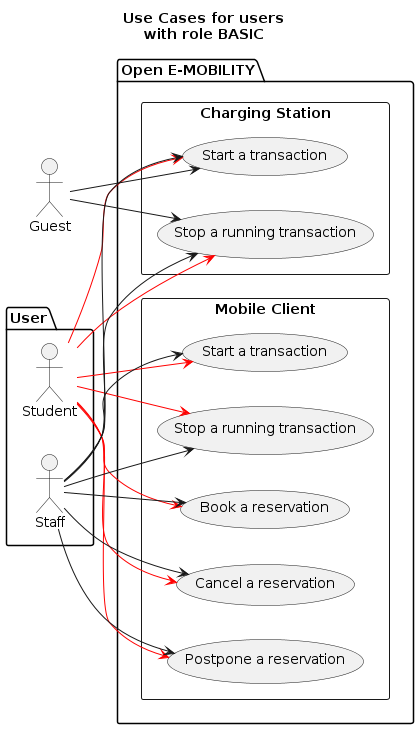
\includegraphics[scale=0.4]{thesis/sections/images/main/2_chapter/uc_basic_users.png}
    \caption{Use Cases for users of Open E-MOBILITY system with role BASIC or as guest user}
    \label{fig:uc_basic_users}
\end{figure}



\begin{figure}[h!]
    \centering
    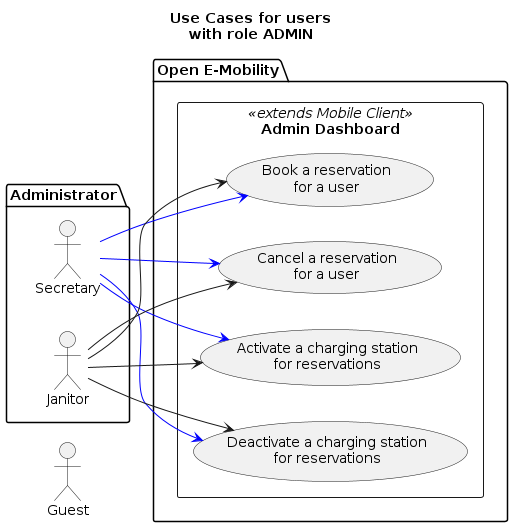
\includegraphics[scale=0.4]{thesis/sections/images/main/2_chapter/uc_admin_users.png}
    \caption{Use Cases for users of Open E-MOBILITY system with role ADMIN or as guest user}
    \label{fig:uc_admin_users}
\end{figure}

\begingroup
\setlength{\tabcolsep}{10pt} % Default value: 6pt
\renewcommand{\arraystretch}{1.5} % Default value: 1
\begin{table}[h!]
    \centering
    \begin{tabular}{m{3.5cm}|c|m{3cm}|m{4cm}}
        Use Case & Shortage & Corresponding Persona & Description \\
        \hline
        Book a reservation & UC1 & Student, Staff, Janitor, Secretary & TODO: \\
        Cancel a reservation & UC2 & Student, Staff, Janitor, Secretary & TODO: \\
        Edit a reservation & UC3 & Student, Staff, Janitor, Secretary & TODO: \\
        Start a transaction & UC4 & Student, Staff, Janitor, Secretary & TODO: \\
        Stop a running transaction & UC5 & Student, Staff, Janitor, Secretary & TODO: \\
        Book a reservation on behalf of another user  & UC6 & Student, Staff, Janitor, Secretary & TODO: \\ 
        Cancel a reservation on behalf of another user & UC7 & Janitor, Secretary & TODO: \\
        Enable charging station for reservation & UC8 & Janitor, Secretary & TODO: \\
        Disable charging station for reservation & UC9 & Janitor, Secretary & TODO: \\
    \end{tabular}
    \caption{Use Case overview with assignment to the corresponding personas and a brief description}
    \label{tab:use_case_overview}
\end{table}
\endgroup

\subsection{System Interactions}
\label{ch:Requirements Engineering and Process Design:sec:Scenario:ssec:System Interactions}

\subsection{Process Design}
\label{ch:Requirements Engineering and Process Design:sec:Scenario:ssec:Process Design}


%% LaTeX2e class for student theses
%% sections/content.tex
%%
%% Karlsruhe University of Applied Sciences
%% Faculty of  Computer Science and Business Information Systems
%%
%% --------------------------------------------------------
%% | Derived from sdqthesis by Erik Burger burger@kit.edu |
%% --------------------------------------------------------

\chapter{Implementation}
\label{ch:Implementation}

\dots
%% LaTeX2e class for student theses
%% sections/content.tex
%%
%% Karlsruhe University of Applied Sciences
%% Faculty of  Computer Science and Business Information Systems
%%
%% --------------------------------------------------------
%% | Derived from sdqthesis by Erik Burger burger@kit.edu |
%% --------------------------------------------------------

\chapter{Analysis and Validation}
\label{ch:Analysis and Validation}

\dots

% Conclusion 
%% LaTeX2e class for student theses
%% sections/conclusion.tex
%%
%% Karlsruhe University of Applied Sciences
%% Faculty of  Computer Science and Business Information Systems
%%
%% --------------------------------------------------------
%% | Derived from sdqthesis by Erik Burger burger@kit.edu |
%% --------------------------------------------------------


\chapter{Conclusion}
\label{ch:Conclusion}

\dots



%% --------------------
%% |   Bibliography   |
%% --------------------

%% Add entry to the table of contents for the bibliography
\printbibliography[heading=bibintoc]


%% ----------------
%% |   Appendix   |
%% ----------------
\appendix
%% LaTeX2e class for student theses
%% sections/apendix.tex
%%
%% Karlsruhe University of Applied Sciences
%% Faculty of  Computer Science and Business Information Systems
%%
%% --------------------------------------------------------
%% | Derived from sdqthesis by Erik Burger burger@kit.edu |
%% --------------------------------------------------------



\iflanguage{english}
{\chapter{Appendix}}    % english style
{\chapter{Anhang}}      % german style
\label{chap:appendix}


%% -------------------
%% | Example content |
%% -------------------
\section{First Appendix Section}
\label{sec:appendix:FirstSection}

\setcounter{figure}{0}

\begin{figure} [ht]
  \centering
  \missingfigure{A figure}
  \caption{A figure}
  \label{fig:anotherfigure}
\end{figure}


\dots
%% ---------------------
%% | / Example content |
%% ---------------------


\end{document}
